\documentclass{article}
\usepackage[utf8]{inputenc}
\usepackage[a4paper, width=160mm, top=20mm, bottom 20mm]{geometry}
\usepackage{graphicx}
\usepackage{float}
\usepackage{ulem}
\usepackage{forest}
\usepackage{tikz}
\usepackage[toc,page]{appendix}
\usepackage{color}
\usepackage{soul}

\usetikzlibrary{positioning}

\newcommand{\wrap}[1]{\parbox{1\linewidth}{\vspace{1.5mm}#1\vspace{1mm}}}


\setlength{\textheight}{25.7cm}
\setlength{\textwidth}{16cm}
\setlength{\unitlength}{1mm}
\setlength{\topskip}{2.5truecm}
\topmargin 260mm \advance \topmargin -\textheight
\divide \topmargin by 2 \advance \topmargin -1in
\headheight 0pt \headsep 0pt \leftmargin 210mm \advance
\leftmargin -\textwidth
\divide \leftmargin by 2 \advance \leftmargin -1in
\oddsidemargin \leftmargin \evensidemargin \leftmargin
\parindent=0pt

\frenchspacing

\usepackage{microtype}
\usepackage[english]{babel}
\usepackage{listings}
\newcommand{\mylanguage}{english}


\title{Design Document}
\author{Beatrice-Andreea Vizuroiu, Cody Boon, Elena Martellucci, Kalle Struik, Mehmet Alp Sozuduz }
\date{March 2021}

\usepackage{natbib}

\begin{document}

    \maketitle

    \section{Introduction}
    This design document follows the OOP Project assigned in 2021, which involves a question and answer system for lecturers to receive questions from their students during (online) lectures. To better understand what the stakeholders want and how to implement them we will discussing it in the following responsible CS and Human Computer Interaction respectively.


    \section{Responsible CS}
    "In what way would our design process and final product change if we also had to design our product for one additional value of a 'non-obvious' stakeholder?" That is the question that we have to ask ourselves when creating a product.\\
    \\We start by defining eight stakeholders\\
    \begin{center}
        \begin{tabular}{ | l | l | l | l | l |}
            \hline
            Direct    & Indirect \\ \hline \hline
            Client  & Anyone else on the same bandwidth/with the same API  \\ \hline
            Lecturer  & Other Students working on the same product  \\ \hline
            TA  &  Competitors  \\ \hline
            Students  & Government  \\ \hline
            Tu Delft  &   \\ \hline
        \end{tabular}
    \end{center}

    The chosen stakeholder in which we will focus on is the \textbf{TU Delft} institution. This is because all the users and systems have to follow its rules and regulation.\\

    A list of three ethical values that we presume important to TU Delft, in the context of an online system that students can ask questions on, are Privacy, House Rules and Code of Ethics.\\

    Privacy, as stated in the Student charter 2020-2021 (in regards to TUDelft) means that "Your personal data can only be accessed by TU Delft staff who are directly or indirectly involved with student administration."\citep{TUDelftMan} TU Delft also outlines a number of legal rights, such as: right of inspection, right to rectification and supplementation, right to object, right to data portability, right to be forgotten, right to restriction of processing and right to file a complaint. Therefore as a product designed to be used within the TU Delft ecosystem we need to assure that it follows the whole protocol.\\

    House rules and disciplinary measures, specifically regarding the use of Educational ICT Facilities, there are some rules that students have to follow when using it. Examples are using a falsified identity, use for educational purposes and  the violation of copyright and intellectual property rights. This is important because a large number of students may be using these facilities when using the program, therefore the program has to adhere to these regulations.  \citep{TUDelftICT}\\

    Code of Ethics means that all members of the TU Delft have to follow one, which includes but is not limited to what to do if you see behaviour that you consider to be inappropriate or (in more serious cases) what to do if you see someone breaking any of the rules stated above. \citep{TUDelftMan}\\

    To find a definition of privacy in the context of a forum in which students can ask questions, it is first important to understand the difference between \textbf{the right of privacy} and \textbf{private information}. The right of privacy is a legal definition that requires the ability to keep personal life secret if the person wishes so, this encompasses  personal information/activities/spaces. Therefore the information privacy is a subsection of the right of privacy, which in the context of a forum means that users have personal information that they don't want to be shared outside the approved community. \citep{PrivacyComputing}\\

    A good example that closely relates to what we are doing are online forums. More specifically an online tool which is very similar to our product is Pigeonhole Live.\citep{pigeonlab}  Within that we can look at their privacy settings, such as the fact that they allow users to remain anonymous if they so wish. This links directly to TU Delft's legal "right to object"\citep{TUDelftMan}. Other resources that could be looked into would be cyber security experts who have specifically work with universities and their need for data privacy. \\

    he following figure is the Values Hierarchy of the chosen ethical value (i.e.Privacy) \\

    \begin{figure}[h]
        \centering
        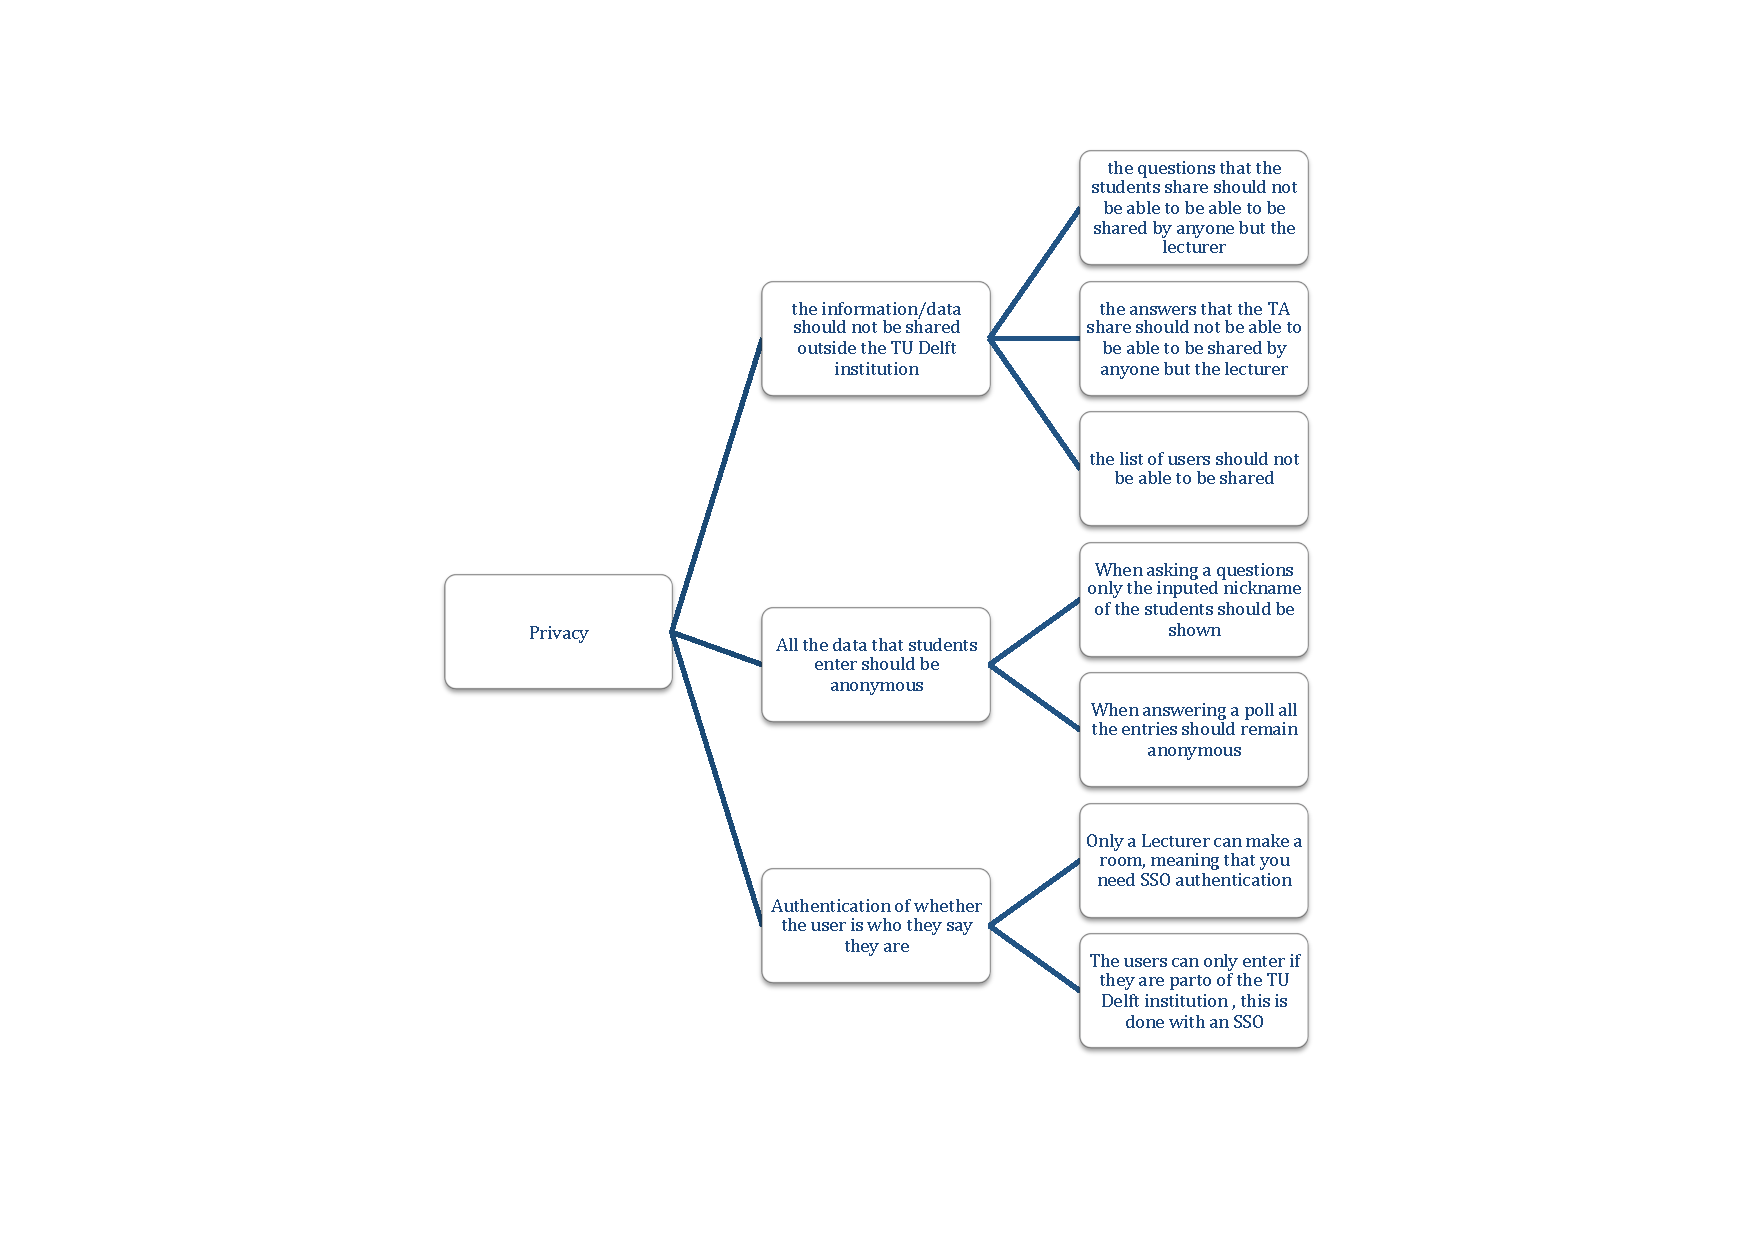
\includegraphics[width=0.9\textwidth]{Responsible CS_tree_v2.pdf}
        \caption{Values Hierarchy showing from left to right the value (i.e. privacy), norms and design requirements..}
        \label{fig:tree}
    \end{figure}


    The design changes that are required to account for the additional value/stakeholder will create issues, specifically regarding \textbf{authentication}. This is because the client (stakeholder 1) and the TU Delft (stakeholder 4) have value tensions. This means that they have contradicting notions in the value themselves. \\

    In this case the client specified that authentication is a "won't have" due to the difficulty working with bureaucracy and not having enough resources to implement it. Moreover, the biggest problem is with time, simply put there isn't enough of it to work on something as important as authentication. In contrast, TU Delft prioritises privacy, therefore not having proper authentication will cause problems in the long run. Specifically if we want to implement the program within the TU Delft ecosystem. This issue will be resolved if we are tasked to continue working on it, but in the current time frame authentication will not be possible to implement.\\

    It is though, important to think about the the moral values which we assume all users must have when not implementing a form of authentication. These values include honesty and integrity such that students will not utilize the application besides it's intended use (e.g. not create their own room). And that TA's have the moral value of respect in regards to the lecturer and do not overstep their bounds (e.g. end the lecture before the lecturer says so).\\

    Overall learning what a less obvious stakeholder requires, allowed us to implement and think about elements which we would not have thought about, specifically the ethical values privacy allowed us to think about the possibility of including self generated usernames if the user does not want to input their own and how certain actions (e.g. polling) may need to remain anonymous. This was all found through doing research on the stakeholder and their rules and regulations. Lastly we also looked beyond the academic sphere and discussed the moral values which we expect the different users oblige by.\\



    \section{HCI}

    The objective of this Human Computer Interaction evaluation is to better understand our strengths and weaknesses in the design of our product. As of the 14\textsuperscript{th} March we have designed a UI that encompasses all the different types of users and what they will see. We also designed an entry page, so that all the different users can be sent to their appropriate views.\\

    \subsection{Methods}
    \subsubsection{Experts}
    Currently, the experts that evaluate our application are made up of 5 students (from group 6) that all have around half-year experience each. It can be argued that these "experts" should actually be considered novices, nevertheless all these students are working on the same project with the same requirements. Therefore they should be very well informed on this specific product and its' requirements. From now on we will refer to them as CS students.\\

    \subsubsection{Procedure}
    To begin, we instructed the experts on what to do by giving them the following instructions:
    \begin{itemize}
        \item Download the Heuristics Evaluation document.
        \item Review the views on the Figma platform.
        \item Grade the questionnaire at the bottom of the document from 1 - 10.
        \item For any additional notes (can't find button etc.), you can simply note them down.
    \end{itemize}
    When referring to the Figma in the instructions, it refers the evaluators to our design on a platform called Figma. Figma is a graphics editor, wherein the designers can link different frames together to emulate what happens when a user clicks on a a certain button. This allows the evaluators, to get a complete experience of what the product should do. This allows us, as designers, to see if there is a problem within the actual design, before coding it.\\

    It is important to note that the contents of the Heuristics Evaluation document include the heuristics, the steps to follow and the questionnaire.\\

    The heuristics which the experts should take into account while analyzing the design are:
    \begin{itemize}
        \item \textbf{Match between system and the real world} = the product should use language and concepts with which the user is familiar with, making sure to avoid any technical jargon  \citep{2Heuristic}
        \item \textbf{Aesthetic and minimalist design}= the interface should only include information which is relevant. Anything else would compete with it and diminish their "relative visibility"\citep{MainHeuristic}
        \item \textbf{Consistency and standards} = Follow not only the industry standards and conventions but also those already placed on the product \citep{MainHeuristic}
        \item \textbf{User control and freedom} = Users should be able to perform mistakes or unwanted actions and easily make their way back to where they were before  \citep{MainHeuristic}
        \item \textbf{Visibility of system status} = The users should always be able to see what is going on in regards with the system. And this should all be shown within a reasonable amount of time \citep{MainHeuristic}
        \item \textbf{Error prevention} = The design should prevent errors from occurring as much as possible. This can be done with giving users a confiramtion message when doing something that can't be undone.   \citep{MainHeuristic}
        \item \textbf{Recognition rather than recall} = make sure that the user does not have to memorize all the elements by making the options visible  \citep{MainHeuristic}
        \item \textbf{Flexibility and efficiency of use} = the program should have ways to speed up interactions for users who are experts or maybe more frequent users. This may be done through shortcuts or settings to tailor frequent actions  \citep{MainHeuristic}
        \item \textbf{Help users recognize, diagnose, and recover from errors} = Error messages should be simple and easy to understand, wherin it indicates the problem and suggests a solution \citep{MainHeuristic}
        \item \textbf{Help and documentation} = Add the proper documentation so that users are better able to understand the system when making use of the program for the first time. \citep{MainHeuristic}
    \end{itemize}
    The evaluators were given the following steps to help them navigate the system:
    \begin{enumerate}
        \item As a student, try to up-vote a question.
        \item As a student, try to ask a question.
        \item As a student, try to tell the lecturer if he/she is too slow/fast.
        \item As a student, try to leave a room.
        \item As a student, try to sort the questions by.
        \item As a lecturer, try to create a room.
        \item As a lecturer, try to export the questions.
        \item As a lecturer, try to mark a question as answered.
        \item As a TA, try to answer a question.
        \item As a TA, try to ban a student from the room.
        \item As a TA, try to create a poll.
    \end{enumerate}
    These steps were chosen because they allow the evaluators to not only see an entire overview of the product but also makes them come across different heuristics. Which will then be discussed in the following sections with the specific questions that were asked.

    \subsection{Measures (data collection)}
    After performing all the tasks the evaluators are asked to answer the following questions by giving an answer ranging from 1 to 10 (1 being very bad and 10 being very good) and add notes to explain their reasoning:
    \begin{enumerate}
        \item How clear is the system status?
        \item How consistent is the design of the application?
        \item How aesthetic yet simplistic is the design of the application?
        \item How easy is it to explore the functionalities of the application?
        \item How easy is it to recognize the functionality of every button?
        \item How efficient is the application?
        \item How easy is it to commit errors (ex. clicking the wrong button)?
        \item How easy is it to recognize and recover from an error (ex. clicking the wrong button)?
        \item How much help does the user receive to understand all the functionalities?
        \item How much do you see yourself using this application?
    \end{enumerate}
    At the end of the questionnaire they were encouraged to add any comments or suggestions that could help us, designers, improve our application design.\\

    All of this has been sent in the Heuristics Evaluation document, and when the experts have finished it they send it back to us, designers. We chose this format because it would be easier for the experts to add any comments throughout the questionnaire if they wish to do so.\\

    Note that we didn't give the experts the specific heuristic for which each question applied to. This was done so that the student experts have very simple and easy to understand questions. But the heuristics will be further discussed in the results to better understand what and how to fix any problems we might encounter.\\

    \subsection{Results}
    The following table report the results given by the 5 experts. Note that each question refers to a specific heuristic, which is important to keep in mind when analysing the results.
    \begin{center}
        \begin{tabular}{|c|c|c|p{0.6\linewidth}|}
            \hline
            Question & Heuristic & \multirow{\parbox{2cm}{\centering Result (average)}} & Comments \\ \hline
            1 & \multirow{\parbox{2cm}{\centering Visibility of system status}} & 5.4 & \wrap{- Not a lot of feedback on the system status \\ - Add a green dot anywhere or something similar to indicate a connection. \\ - No status bar but can see if the system is functioning } \\ \hline
            2 &\multirow{\parbox{2cm}{\centering Consistency and standards}}& 9.0 & \wrap{- A question that I hadn’t yet up-voted was already purple \\ - System is very consistent overall and in the main design there are no differences between screens \\ - The font and size of the button/text/... vary between screens and I had to zoom/de-zoom to properly see
            everything.} \\ \hline
            3 &\multirow{\parbox{2cm}{\centering Aesthetic and minimalist design}}& 7.6 & \wrap{-Lot of icons that make it less simplistic \\ - It’s pretty simple but sometimes there is a lot going on in the options bar\\ - Improve the sizing and distribution of the top right buttons \\ - A lot of icons sometimes in the right corner above makes it a little more complicated } \\ \hline
            4 &\multirow{\parbox{2cm}{\centering User control and freedom}}& 6.0 & \wrap {- It’s hard to explore because there are no back buttons. \\ - It is mainly clear how everything works, since there is only one sub menu and there is a big question mark if you want to know what everything does \\ - I couldn’t always find the features mentioned in this document. (sorting the questions, leaving the room and answer a question) } \\ \hline
            5 &\multirow{\parbox{2cm}{\centering Recognition rather than recall}}& 9.2 & \wrap{- All of the symbols are common symbols so you know what to expect. Except the “export question” symbol. \\ - Except for maybe the upvote button, which could be unclear for someone not familiar, everything is quite easy to recognize. There are labels everywhere and where there are no labels, there is no need.} \\ \hline
            6 &\multirow{\parbox{2cm}{\centering Flexibility and efficiency of uses}}& 8.0 & \wrap{- Most buttons are available with very few clicks. \\ - It is  not possible to schedule a lecture  \\ - Sometimes close functions such as timeout and ban, for example only after clicking on something else since banning doesn’t happen too often} \\ \hline
            7 &\multirow{\parbox{2cm}{\centering Error prevention}}& 5.0 & \wrap {- Easy to commit errors and there is no “back” button. You could also make a different colour for text fields and buttons, that way it’s more clear.\\ - It is extremely easy to commit to an error since there is no prompt when for example deleting a question.} \\ \hline
            8 &\multirow{\parbox{2cm}{\centering Help users recognize, diagnose, and recover from errors}}& 4.4 & \wrap {- No real error messages or back button to get out of a certain situation \\ - Not very easy to find an exit/back button \\ - There is not really a possibility to see what you have done and no return button, so to recover from an error is not possible. } \\ \hline
            9 &\multirow{\parbox{2cm}{\centering Help and documentation}}& 7.6 & \wrap { \\ - There is a question mark but it’s not really clear what happens if you click on this \\ - I am not sure how good the help button is, but I would think that gives all the help someone may need}\\ \hline
            10 &\multirow{\parbox{2cm}{\centering Overall}}& 8.6 &  \\ \hline
        \end{tabular}
    \end{center}

    Note that the results show the average of the raw data. The raw data is taken from 5 experts, therefore it is calculated using the following equation:
    \[ \frac{(r_1 + r_2 + r_3 + r_4 + r_5)}{5} = average \]
    Where r is the result and the number below indicates which user it is from 1 to 5.
    \\

    Along with the results we were given comments for each question (see table) and also general comments. It is important to note that the table mostly includes the comments in which tips are given and not the ones that say, for example, "good simplistic design". This is because the tips are constructive feedback that help us find what we should specifically fix. The general comments are:
    \begin{itemize}
        \item In general, it’s a nice, intuitive design. However, it was hard to tell how to join as a moderator or student. It would be useful to make this more clear.
        \item It looks good. The link in the moderator view (I think?) is not functioning clearly, I couldn't tell what it does, and it is not very clear how the feedback works. For example, can a user click as many times as they want or do you stay on too slow or too fast (is it continuous feedback?), if so maybe there could be an option for not too slow or too fast, but just right.
        \item It looks really good already, maybe make it more clear when you’re in a student or moderator view, I couldn’t tell. I also didn’t completely understand the difference between the faster and slower buttons as opposed to the circles with too fast too slow but maybe that’s just the student and moderator view. (Lecturer / student difference) Maybe somewhere provide information on what it means to timeout a user (e.g. how long does this last?). Other than that nice job!
        \item Overall, it’s a pretty amazing application, you have used features such as hovering, highlighting the correct features, dark mode, ... which are quiet advanced and it really looks like a professional app! Here are some remark I had when testing the app.
        \begin{itemize}
            \item When sending a question, the icon for the light/dark mode change position.
            \item When creating a new “room” the user is asked to enter the name of the lecturer, I don’t think this is really necessary if the students are also allowed to create room (the course id is sufficient I think, people good start messing around with the lecturer’s name and this could become offensive).
            \item You did not include anything about the time/date of the lecture, are you planning on doing so?
        \end{itemize}
    \end{itemize}
    As you can see, the three questions wherein we have the lowest results are (going from lowest) are question 8, 5 and 1. These refer to the heuristics: Help users recognize,diagnose,and recover from errors, Recognition rather than recall and Visibility of system status.  The reason why and how we are going to improve it will be discussed in the Conclusion and Improvements.\\

    Overall, there were also no major outliers in the data and the global trend shows that the experts enjoyed using the application.


    \subsection{Conclusions and Improvements}
    To conclude, these results show that the overall design of the application is very good with few problems here and there (specifically regarding the how recognizable buttons are(i.e. question 5)).There also seems to be notable problems regarding error notification and the status of the system (question 8 and 1 respectively).\\

    Advice regarding these two problems, that were given by the experts, include: \begin{itemize}
                                                                                      \item Adding error messages to the UI.
                                                                                      \item Including back buttons to be able to recover from an error or unwanted action
                                                                                      \item Including a confirmation pop-up when doing something permanent (e.g. a student deleting a question)
                                                                                      \item Giving feedback that denotes system status. I.e. green light to show the system is functioning correctly.
    \end{itemize}

    Those were a few tips from experts on how we could improve our lowest scoring points.\\

    The main problems with our design are omitting necessary information, lack of confirmation/notification when performing permanent actions, and absence of "back" buttons (that allow recovery from errors or unwanted actions).\\

    To account for the first problem, we could introduce an indicator signal that will show the system status. Another way of showing this information could be through adding explicit messages when something happens (e.g. error or crash).\\

    For the second problem,specifically regarding confirmation and notification.The introduction of pop-up buttons as advised from our student experts could be a good idea.  Although  we believe that these do not align with the intention of our app - a side application that lecturers and students will use to communicate efficiently their questions and answers without distraction from the lesson.\\

    For the last point, simply adding "back" buttons as recommended should solve this issue.
    There are a few more less urgent remarks, such as the fact that some buttons are less recognizable than others. If time allows it, we are planning to discus and change them and even adding shortcuts.\\

    Overall, the heuristics, specifically the aesthetic and minimalist design and consistency and standards, data shows that our overall design is minimalist and consistent. It was, generally, received well by the experts that we contacted. They have given us a few points to work on and improve. We hope that through this heuristic evaluation, our app will become easier to understand and use. \\

    Note that all the advice that were taken from the student experts and applied to the design can be seen in the final GUI appendix \ref{appendix:GUI}.

    \section{Conclusion}
    Overall the Responsible CS and the Human Computer Interaction allowed us to better understand what our product should include. This all in regards to what the stakeholders want and figuring out whether or not it works with within our design. Which brings us to our optimal design (See GUI appendix \ref{appendix:GUI})


    \bibliographystyle{plain}
    \bibliography{references}


    \begin{appendices}

        \section{Final GUI}
        \label{appendix:GUI}
        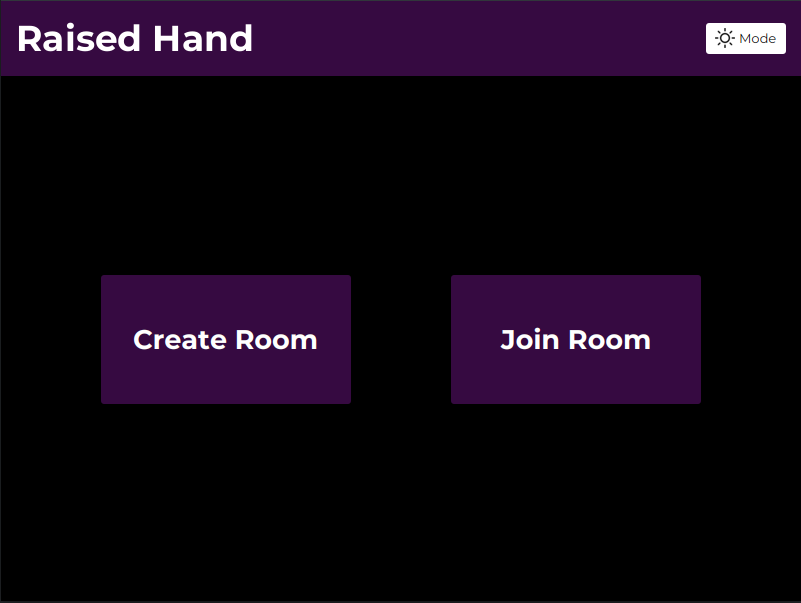
\includegraphics[scale=0.6]{Entry.png}\\
        Figure 2: Entry Page (Dark mode)\\
        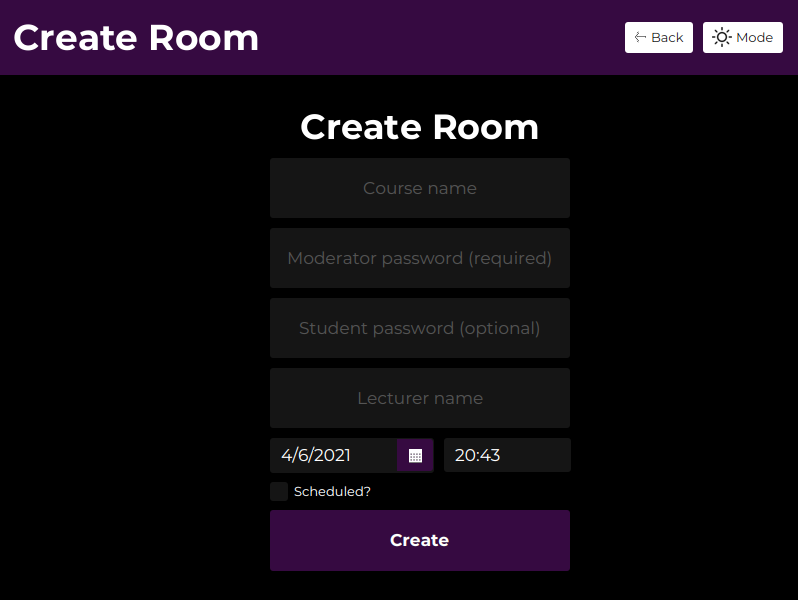
\includegraphics[scale=0.6]{Create.png}\\
        Figure 3: Create Page (Dark mode)\\
        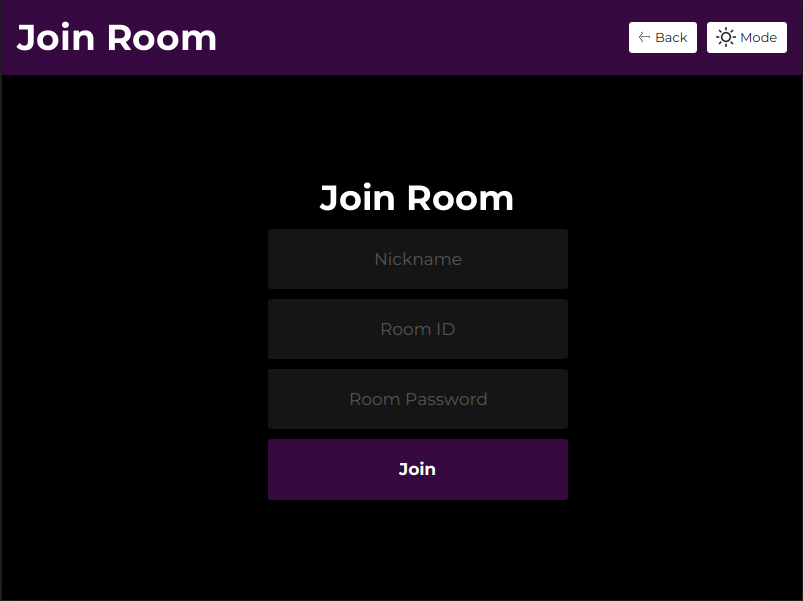
\includegraphics[scale=0.6]{Join.png}\\
        Figure 4: Join Page (Dark mode)\\
        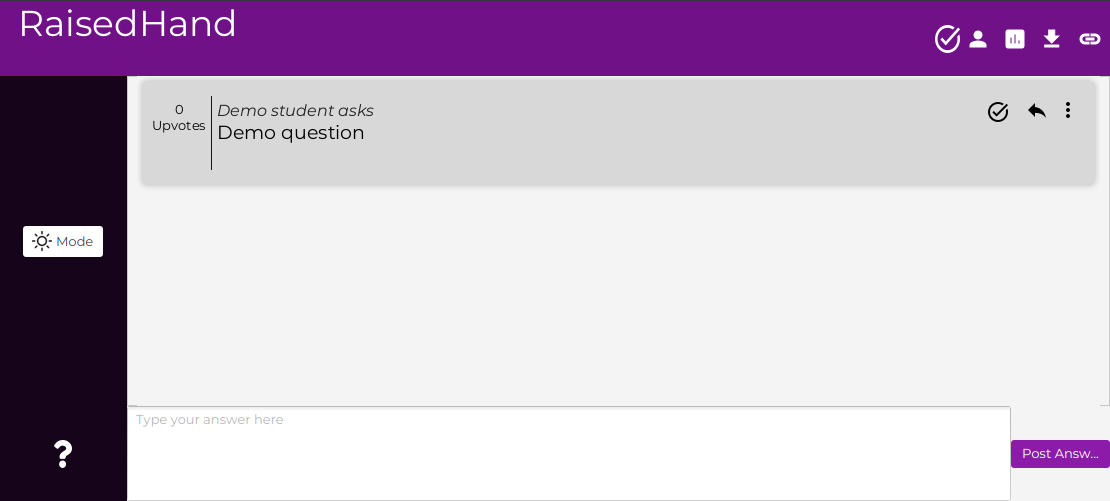
\includegraphics[scale=0.5]{Lecturer_view.png}\\
        Figure 5: Lecturer View (Light mode)\\
        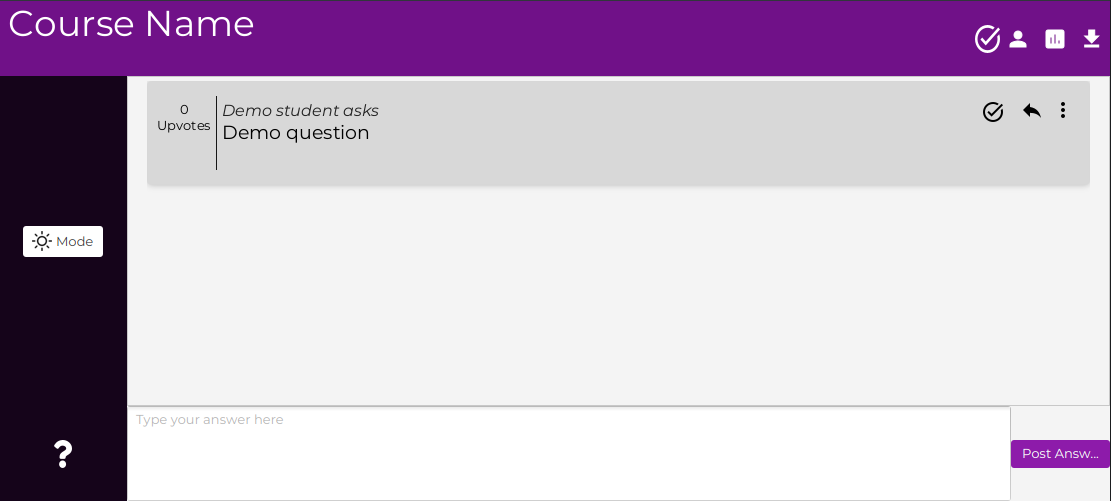
\includegraphics[scale=0.5]{TA_View.png}\\
        Figure 6: TA View (Light mode)\\
        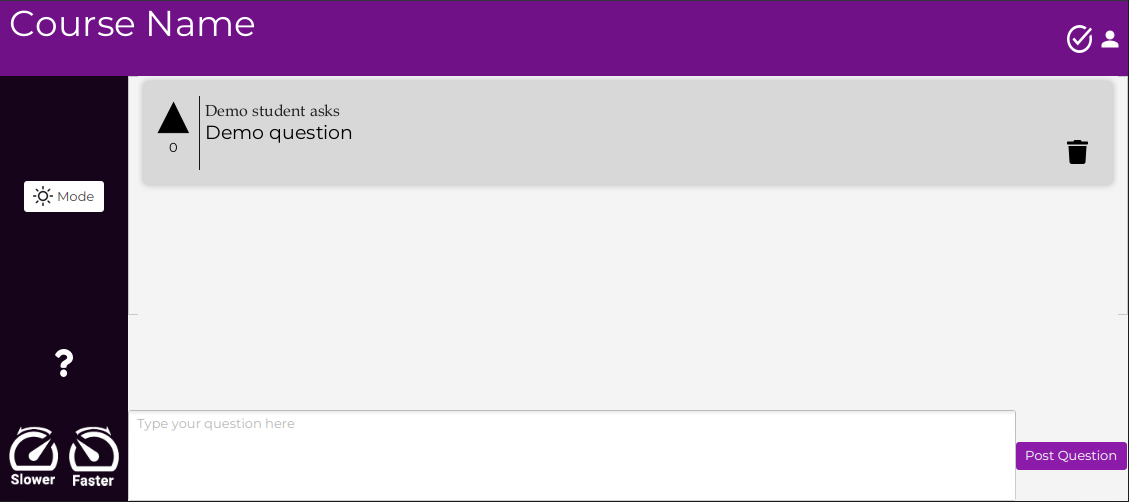
\includegraphics[scale=0.5]{Student_view.png}\\
        Figure 7: Student View (Light mode)\\
        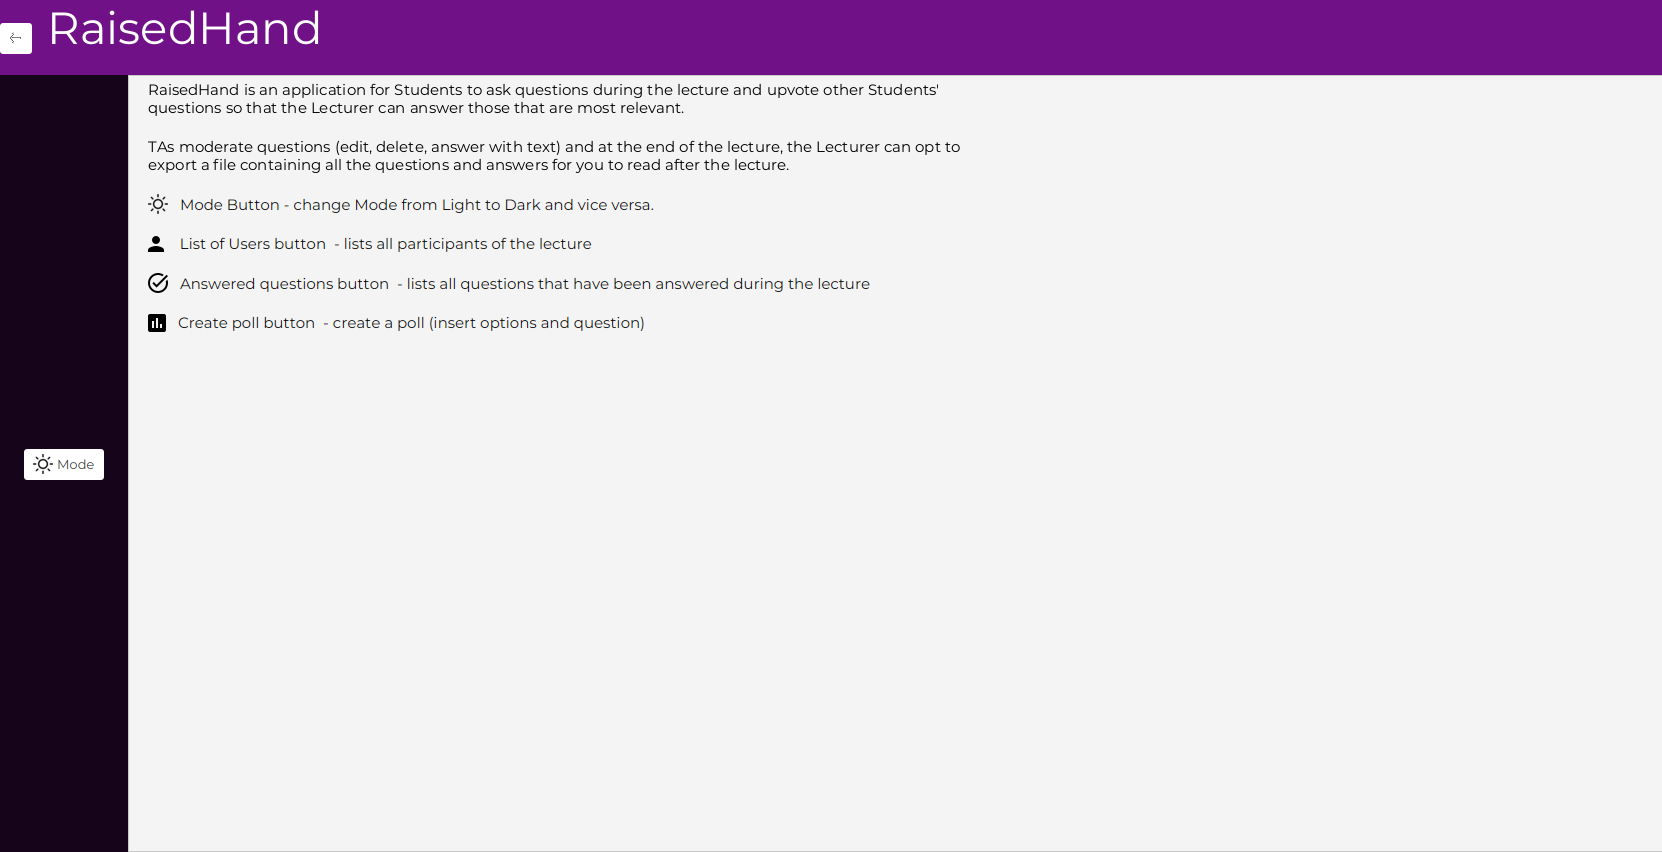
\includegraphics[scale=0.4]{Mod_help.png}\\
        Figure 8: TA View of the Help button (Light mode)\\

        \section{Questionnaire}
        \label{appendix:Questionnaire}
        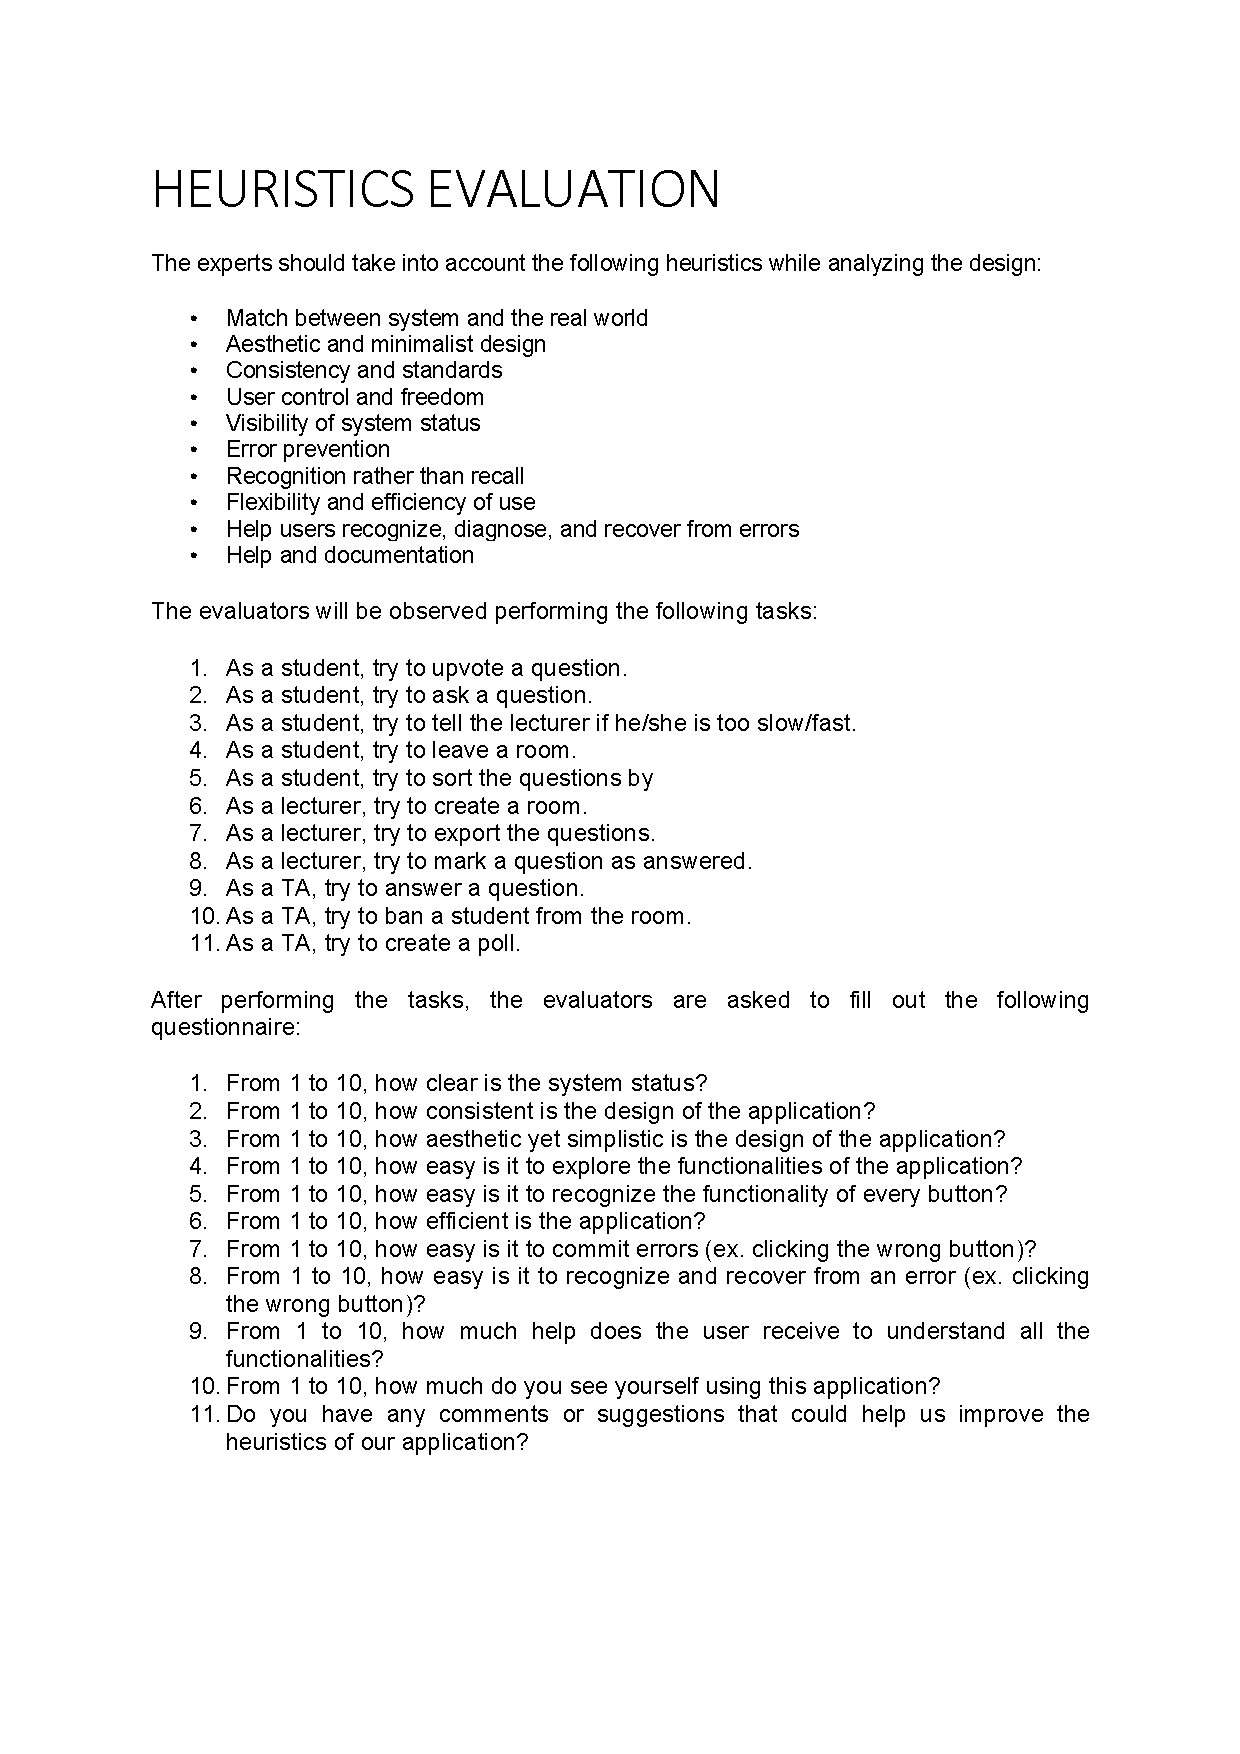
\includegraphics[scale=0.8]{Heuristics_Evaluation_-_eu.pdf}\\



    \end{appendices}
\end{document}